%!TEX root = ../template.tex
%%%%%%%%%%%%%%%%%%%%%%%%%%%%%%%%%%%%%%%%%%%%%%%%%%%%%%%%%%%%%%%%%%%
%% chapter1.tex
%% NOVA thesis document file
%%
%% Chapter with introduction
%%%%%%%%%%%%%%%%%%%%%%%%%%%%%%%%%%%%%%%%%%%%%%%%%%%%%%%%%%%%%%%%%%%

\typeout{NT FILE chapter1.tex}%

\chapter{Introduction}
\label{cha:introduction}

\prependtographicspath{{Chapters/Figures/Covers/}}

% epigraph configuration
\epigraphfontsize{\small\itshape}
\setlength\epigraphwidth{12.5cm}
\setlength\epigraphrule{0pt}


% ................... MOUSE LOCOMOTION .................................................
\section{Mouse locomotion}
\label{sec:getting_started}

\subsection{Cerebellar contributions to coordinated movement}
\label{sub:using_overleaf}

\ntindex[Cerebellar!layers]{}
\ntindex[Cerebellar!cell types]{}


% ................... THE CEREBELLAR CIRCUIT ...........................................
\section{The cerebellar circuit}
\label{sec:cb_circuit}

\subsection{Cerebellar cortex and the Deep Cerebellar Nuclei}
\label{sub:cv_ctx_dcn}

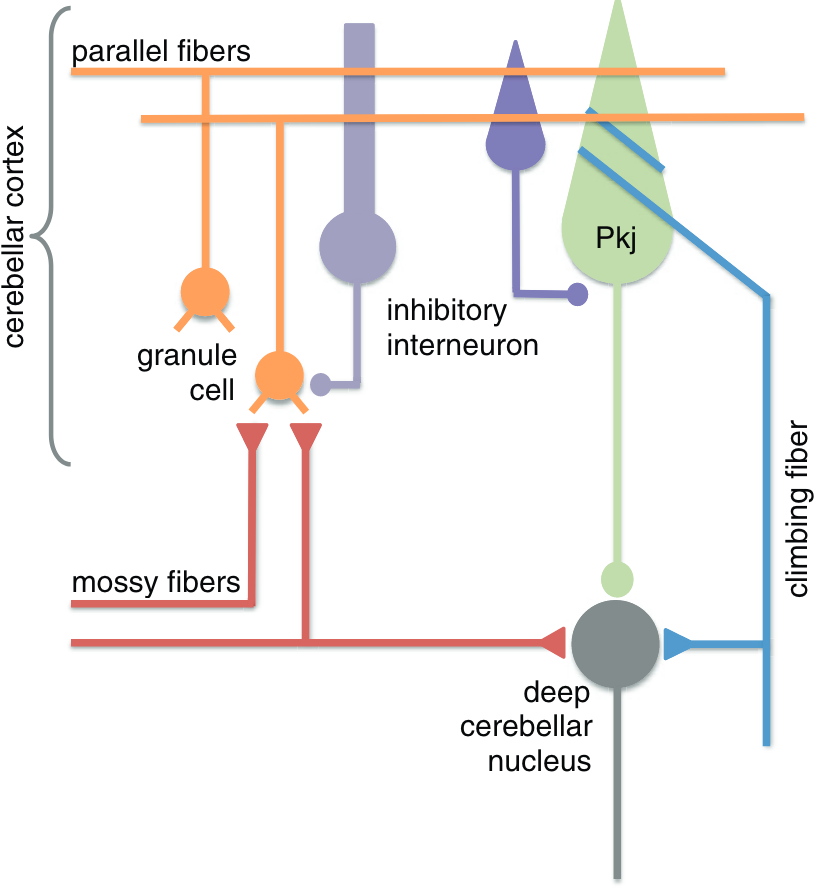
\includegraphics[width=5cm]{Chapters/Figures/chapter1/placeholder_ch1_1_circuit.png}

\subsection{Cerebellar layers}
\label{sub:cb_layers}

\subsection{Cell types}
\includegraphics[width=12cm,height=3cm]{example-image-a}

% ................... CEREBELLAR FUNCTION ...........................................
\section{Cerebellar function}
\label{sec:cb_function}

\subsection{Cerebellar function in health and disease}
\subsection{Movement modulation and learning in Purkinje cells}


% \newcommand{\Overleaf}{\href{https://www.overleaf.com?r=f5160636&rm=d&rs=b}{Overleaf}}

% \begin{wrapfigure}{r}{0.3\linewidth}
% % \vspace*{-10ex}
% \includegraphics[width=\linewidth]{overleaf}%
% \caption{NOVAthesis template in Overleaf.}
% \label{fig:overleaf}
% \end{wrapfigure}


